\documentclass{article}
\usepackage[a4paper]{geometry}

\usepackage[utf8]{inputenc}
\usepackage{amsmath}
\usepackage{hyperref}
\usepackage{listings}
\usepackage{xcolor}
\usepackage{graphicx}
\usepackage{float}

\lstdefinestyle{python}{
language=Python,
basicstyle=\ttfamily\small,
keywordstyle=\color{blue}\bfseries,
stringstyle=\color{red},
commentstyle=\color{green!50!black},
showstringspaces=false,
breaklines=true
}

\title{Simulación y Análisis de Sistemas de Reparación}
\author{Eduardo Brito Labrada \\ Grupo: C-311 \\ Telegram: @eblabrada}
\date{}

\begin{document}

\maketitle

\section{Introducción}
\subsection{Descripción del Proyecto}

El propósito de este proyecto es simular el comportamiento de un sistema de reparación que requiere mantener operativas $n$ máquinas en todo momento. Para mitigar los efectos de posibles fallos, se cuenta con $s$ máquinas adicionales que actúan como repuestos (spares). El sistema está diseñado de manera que, cada vez que una máquina falla, se sustituye inmediatamente por una máquina de repuesto disponible. La máquina que falló se envía a un taller de reparación donde un único reparador trabaja en ellas de forma secuencial, una a una.

El sistema se considera operativo mientras haya al menos una máquina de repuesto disponible para reemplazar las máquinas que fallen. El sistema \textit{colapsa} o \textit{falla completamente} en el momento en que una máquina en uso falla y no hay repuestos disponibles para su sustitución inmediata.

Inicialmente, hay $n + s$ máquinas funcionales: $n$ de ellas se ponen en operación y $s$ se mantienen como repuestos. El objetivo de la simulación es estimar el valor esperado del tiempo $T$ hasta que el sistema colapsa, es decir, cuando el número de máquinas dañadas supera al número de repuestos disponibles.

Este ejemplo es tomado del libro ``Simulation, Fifth Edition by Sheldon M. Ross'', ejemplo $7.7$.

\section{Detalles de Implementación}

La implementación del sistema de simulación se realizó mediante un enfoque de simulación basada en eventos discretos, utilizando una cola de prioridad para manejar eventos futuros y una lógica centrada en el ciclo de fallos y reparaciones de componentes.

Se define la clase \texttt{RepairSystem}, la cual recibe como parámetros el número de componentes operativos (\texttt{n\_operating}), repuestos disponibles (\texttt{n\_spares}), una función generadora de tiempo hasta fallo, y una función generadora de tiempo de reparación. También puede capturar el estado del sistema a lo largo del tiempo, si se activa el parámetro \texttt{capture\_states}.

\begin{lstlisting}[style=python, caption={Constructor de la clase RepairSystem}]
class RepairSystem:
    def __init__(self, n_operating, n_spares, time_to_breakdown, time_to_repair, capture_states=False):
      
\end{lstlisting}

El sistema maneja dos tipos de eventos: \texttt{BREAKDOWN} (fallo de componente) y \texttt{REPAIR\_COMPLETE} (finaliza la reparación de un componente). Estos eventos se almacenan en una cola de prioridad, de manera que siempre se procesa el evento más próximo en el tiempo.

Cada componente comienza operando, y se programan sus respectivos tiempos hasta fallo al inicio. Cuando un componente falla, si aún hay repuestos disponibles, se sustituye de inmediato y se programa un nuevo fallo. El componente dañado pasa a la cola de reparación. Si no hay reparación en curso, esta comienza inmediatamente. Si ya hay una reparación en proceso, el componente espera en la cola de reparación interna.

\begin{lstlisting}[style=python, caption={Clase Event y manejo de eventos}]
class EventType(Enum):
    BREAKDOWN = "breakdown"
    REPAIR_COMPLETE = "repair_complete"

class Event:
    def __init__(self, time: float, event_type: EventType):
        self.time = time
        self.event_type = event_type
    def __lt__(self, other):
        return self.time < other.time
\end{lstlisting}

El método principal \texttt{run()} ejecuta la simulación hasta que el número de componentes dañados supera el número de repuestos. En ese momento se considera que el sistema ha fallado por completo, y se devuelve el tiempo en que ocurre este evento crítico.

\begin{lstlisting}[style=python, caption={Ejecución del sistema}]
def run(self):
    self.schedule_initial_events()
    while True:
        event = heapq.heappop(self.event_queue)
        self.current_time = event.time
        if event.event_type == EventType.BREAKDOWN:
            self.handle_breakdown()
        else:
            self.handle_repair_complete()
        if self.down > self.n_spares:
            break
    return self.current_time
\end{lstlisting}

Se definieron las siguientes clases clave para representar el modelo:

\begin{itemize}
    \item \texttt{ModelConfig}: encapsula la configuración del sistema con el número de servidores en operación y repuestos, las funciones generadoras de tiempos de fallo y reparación, y una etiqueta descriptiva.
    \item \texttt{CrashTimeAnalysis}: almacena los resultados de simulaciones, incluyendo promedio, desviación estándar, error y tamaño de muestra, y permite una representación legible de estos.
\end{itemize}

Las funciones generadoras de tiempos de fallo y reparación se modelan como variables aleatorias exponenciales con tasas $ \lambda = 1/100 $ (fallo) y $\mu = 1/20$ (reparación), respectivamente.

\begin{lstlisting}[style=python, caption={Definición de configuración del modelo}]
class ModelConfig:
    def __init__(self, n_operating, n_spares, breakdown_gen, repair_gen, label):
        self.n_operating = n_operating
        self.n_spares = n_spares
        self.breakdown_gen = breakdown_gen
        self.repair_gen = repair_gen
        self.label = label
\end{lstlisting}

\subsection{Simulación}
La simulación avanza generando tiempos de fallos y reparaciones para los servidores en operación y en repuesto, siguiendo un esquema de reemplazo inmediato cuando un servidor falla. El proceso termina cuando el sistema no tiene servidores operativos disponibles, momento en que se registra el tiempo total hasta el fallo.

Se realizaron múltiples corridas para obtener distribuciones estadísticas del tiempo hasta el fallo total, con un criterio de parada basado en la precisión del intervalo de confianza del 95\%.

\section{Resultados y Experimentos}
Se realizaron simulaciones para diferentes configuraciones de servidores:

\begin{itemize}
    \item Modelo 1: 5 servidores en operación y 2 repuestos.
    \item Modelo 2: 5 servidores en operación y 3 repuestos.
\end{itemize}

La simulación generó distribuciones de tiempos hasta fallo total que permitieron comparar la robustez del sistema según el número de repuestos disponibles.

\begin{figure}[H]
   \centering
    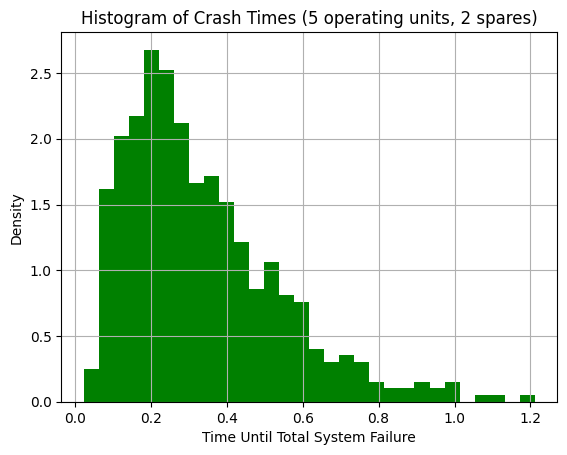
\includegraphics[width=0.8\textwidth]{images/histogram_crash_times1.png}
   \caption{Distribución de tiempos hasta fallo total para Modelo 1 (5 operativos, 2 repuestos).}
\end{figure}

\begin{figure}[H]
   \centering
   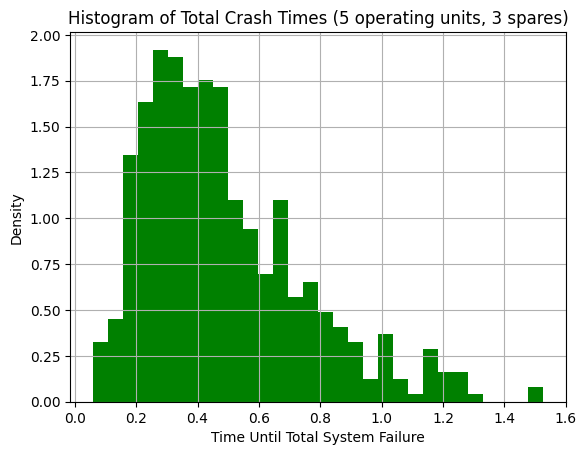
\includegraphics[width=0.8\textwidth]{images/histogram_crash_times2.png}
   \caption{Distribución de tiempos hasta fallo total para Modelo 2 (5 operativos, 3 repuestos).}
\end{figure}

\subsection{Análisis Estadístico y Validación}
Se planteó la hipótesis:

\[
\begin{aligned}
H_0 &: \text{No hay diferencia significativa en el tiempo medio hasta fallo entre los modelos} \\
H_1 &: \text{Existe diferencia significativa en el tiempo medio hasta fallo}
\end{aligned}
\]

Se utilizó un test Z para diferencia de medias con nivel de significancia 5\%, aplicando el siguiente estadístico:

\[
z = \frac{\overline{X}_1 - \overline{X}_2}{\sqrt{\frac{S_1^2}{n_1} + \frac{S_2^2}{n_2}}}
\]

donde $\overline{X}_i$, $S_i$, $n_i$ son la media, desviación estándar y tamaño de muestra para cada modelo.

\begin{figure}[H]
   \centering
   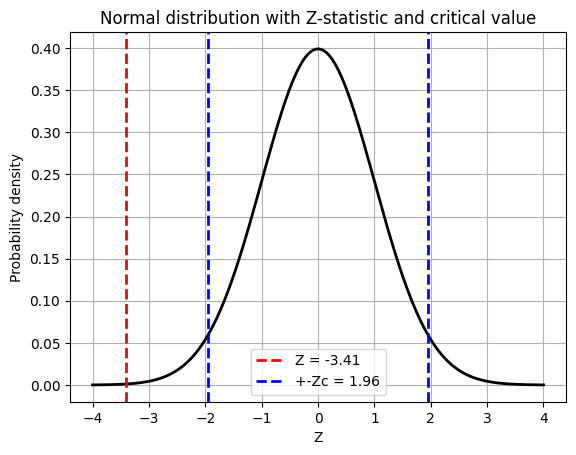
\includegraphics[width=0.8\textwidth]{images/hypothesis_test.png}
   \caption{Prueba de hipótesis para diferencia de medias en tiempos hasta fallo, con intervalo crítico en azul y estadístico en rojo (fuera del intervalo).}
\end{figure}

Dado que el estadístico de prueba se encuentra fuera del intervalo crítico, se rechaza la hipótesis nula. Por lo tanto, existe evidencia estadística para afirmar que hay una diferencia significativa en el tiempo medio hasta fallo entre los modelos comparados.

Este resultado indica que la configuración con mayor cantidad de servidores de repuesto impacta significativamente el tiempo hasta el fallo total del sistema bajo las condiciones simuladas.



Finalmente, se repitió el proceso para otro par modelos, lo cual validó también la hipótesis inicial:

\begin{figure}[H]
   \centering
   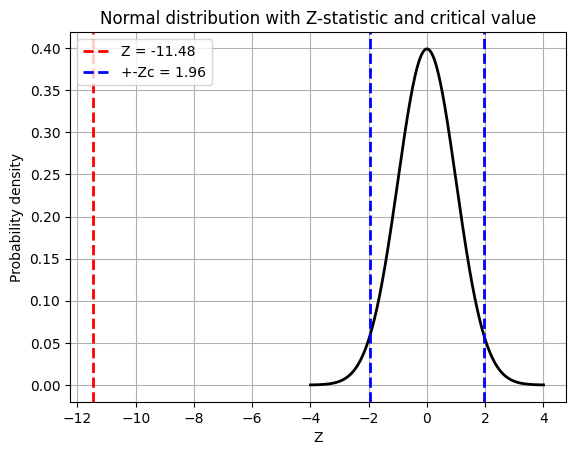
\includegraphics[width=0.8\textwidth]{images/6_1_vs_6_4.png}
   \caption{Prueba de hipótesis para diferencia de medias en tiempos hasta fallo de 6 operativos y 1 repuesto vs. 6 operativos y 4 repuestos, con intervalo crítico en azul y estadístico en rojo (fuera del intervalo).}
\end{figure}


\subsection{Criterio de Parada}
Se usó un criterio basado en intervalos de confianza para asegurar precisión estadística:

\[
2 \times z_{\alpha/2} \times \frac{S}{\sqrt{n}} \leq \text{error aceptado}
\]

donde $z_{\alpha/2}$ es el valor crítico para 95\%, $S$ la desviación estándar de la muestra y $n$ el número de simulaciones. Se corrieron simulaciones hasta cumplir este criterio.

\end{document}
